\chapter{Implementacija i korisničko sučelje}
		
		
		\section{Korištene tehnologije i alati}
		
			%\textbf{\textit{dio 2. revizije}}
			
			 %\textit{Detaljno navesti sve tehnologije i alate koji su primijenjeni pri izradi dokumentacije i aplikacije. Ukratko ih opisati, te navesti njihovo značenje i mjesto primjene. Za svaki navedeni alat i tehnologiju je potrebno \textbf{navesti internet poveznicu} gdje se mogu preuzeti ili više saznati o njima}.
			 \subsection{Tehnologije koje čine aplikaciju}
			 	Aplikacija ima  \href{https://www.djangoproject.com/}{Django} backend i \href{https://react.dev/}{React} frontend te za bazu podataka koristi \href{https://www.postgresql.org/}{PostgreSQL}. Django je web framework za Python koji je dostatan za izradu cijelih web aplikacija jer obuhvaća izradu sučelja putem HTML-a i CSS-a, komunikaciju s bazom podataka i backend logiku u jeziku Python. On s bazom podataka komunicira tako da preslikava Python objekte na bazu (takvi sustavi se još zovu ORM, kratica od Object Relational Mapping). Komunikacija s PostgreSQL bazom podataka se u Django-u ostvaruje korištenjem Python modula \href{https://pypi.org/project/psycopg2/}{psycopg2}. koji omogućuje spajanje na bazu podataka, njenu administraciju te slanje SQL upita poslužitelju baze podataka. To je ujedno i najkorišteniji Python modul za PostgreSQL, a tu je naveden jer ga eksplicitno koristimo u dijelovima aplikacije koji trebaju izvršiti velike upite na bazi podataka. Pri eksplicitnom komuniciranju s bazom, morali smo paziti da koristimo iste module kao i Django, kako ne bi nastali problemi s bazom. Naš tim je odlučio frontend odraditi u React frameworku, a s Django-om odraditi backend i komunikaciju s bazom. React i Django su u aplikaciji spojeni tehnologijom \href{https://www.django-rest-framework.org/}{Django REST framework}, koja omogućuje da oni komuniciraju međusobno. React je frontend web framework koji omogućuje izgradnju web sučelja korištenjem HTML-a, CSS-a i skriptnog jezika Javascript. React-om se najčešće izrađuju web sučelja, ali je moguće izraditi i takozvane desktop aplikacije koristeći tehnologije kao što je Electron. U tom slučaju se React aplikacija izvršava na instanci preglednika Google Chrome te je oblikovana da se ponaša kao ostale desktop aplikacije.
			
			\subsection{Tehnologije za komunikaciju s članovima tima}
				Za komunikaciju među članovima tima smo uglavnom koristili platforme Whatsapp i Discord te u manjem omjeru platforme Telegram i Element. Platformu MS Teams nismo koristili za komunikaciju među članovima tima jer ne podržava dobro preglednik Firefox i desktop aplikacija za operacijski sustav Linux je spora i nespretna za korištenje. Tri člana koriste Linux, a od toga dva imaju samo Linux na računalima. Stoga nam je bitno da svi alati podržavaju i Windows i Linux te da su na oba sustava iskoristivi u jednakom opsegu.
				
			\subsection{Tehnologije za pisanje dokumentacije}
				Pošto je zadano da dokumentaciju izrađujemo u LaTeX-u, a trebala nam distribucija koja podržava i Linux i Windows. odlučili smo se za \href{https://www.tug.org/texlive/}{TeX Live} jer postoji kao paket u repozitorijima modernih Linux distribucija. Za typesetting nam služi editor Texworks, koji je dio TeX Live distribucije. Odabir alata za uređivanje TEX datoteka je ostavljen članovima tima, a neki od odabranih uz TeXworks su: terminal editor \href{https://www.vim.org/}{Vim}, \href{https://code.visualstudio.com/}{Visual Studio Code} napravljen u Electron-u i \href{https://www.sublimetext.com/}{Sublime Text}.
			
			\subsection{Tehnologije za izradu popratnih sadržaja, odnosno dijagrama, grafika i prezentacija}
				Za izradu zadanih dijagrama najviše smo koristili \href{https://www.drawio.com/}{draw.io}, koji omogućuje laganu izradu dijagrama tehnikom drag and drop te sadrži sve potrebne elemente UML dijagrama. Pored toga još sadrži i dijagrame arhitekture strujnih krugova i mnoge druge tipove dijagrama. Međutim, postoje slučajevi kada dijagrame treba doraditi pa smo za to koristili \href{https://inkscape.org/}{Inkscape}, koji manipulira slike u SVG formatu. SVG je grafički format u kojem su slike predstavljene matematičkim formulama, a ne pikselima pa su stoga lako skalabilne bez da gube na razlučivosti. Za potrebe uređivanja slika koristili smo \href{https://www.gimp.org/}{GIMP}, a za skiciranje pri radu smo koristili program \href{https://krita.org/}{Krita}. Prezentacije izrađujemo alatom \href{https://www.libreoffice.org/}{Libreoffice Impress}.
				
			\subsection{Tehnologije za pisanje programskog koda}
				Programi opće namjene kojima smo pisali kod su: terminal editor \href{https://www.vim.org/}{Vim}, \href{https://code.visualstudio.com/}{Visual Studio Code} napravljen u Electron-u i \href{https://www.sublimetext.com/}{Sublime Text}. Pri pisanju Python-a, korišteno je razvojno okruženje \href{https://www.spyder-ide.org/}{Spyder}, a za provjeru frontenda preglednici \href{https://www.mozilla.org/en-US/firefox/new/}{Firefox} i \href{https://www.google.com/chrome/}{Google Chrome}. Koristili smo \href{https://www.pgadmin.org/download/}{pgAdmin4} za upravljanje bazom podataka.
				
			\subsection{Tehnologije vezane za sustav upravljanja inačicama}
				Osim programa Git, koristili smo i popratne alate da nam olakšaju rad na zajedničkom repozitoriju. Članovi na sustavu Linux su koristili \href{https://github.com/prati0100/git-gui/}{git-gui}, to je alat za upravljanje git commit-ovima s grafičkim sučeljem koji je dostupan i na Windows sustavima.	Uz njega je vezan alat gitk,	koji grafički prikazuje repozitorij, grane i povijest commit-ova. Također, on dopušta manipulaciju lokalnom povijesti repozitorija. Članovi na Windows sustavima su koristili \href{https://desktop.github.com/}{GitHub desktop}, koji ima grafičko sučelje. S obzirom da imamo članove na sustavima Linux i Windows koji surađuju, važno je podesiti alate tako da članovi na Windows sustavima u repozitorij šalju datoteke s Unix znakovima za kraj retka.
			\subsection{Sažetak}
				Većina odabranih alata ima javni izvorni kod s licencama koje dopuštaju korisniku da ih kopira, mijenja i distribuira, Izbor alata je posljedica iskustva voditelja projekta u radu s njima, a u namjeri da ostalim članovima može pomoći što više.
			\eject 
		
	
		\section{Ispitivanje programskog rješenja}
			
			%\textbf{\textit{dio 2. revizije}}\\
			
			 %\textit{U ovom poglavlju je potrebno opisati provedbu ispitivanja implementiranih funkcionalnosti na razini komponenti i na razini cijelog sustava s prikazom odabranih ispitnih slučajeva. Studenti trebaju ispitati temeljnu funkcionalnost i rubne uvjete.}
			Napomena: Ispitivanje nije implementirano zbog manjka članova koji rade u timu, što je odvuklo pozornost od testiranja. Međutim, u daljnjem tekstu je objašnjen proces testiranja Python koda.
			
			Za testiranje Python dijelova aplikacije namjeravali smo koristiti Python modul \href{https://docs.pytest.org/en/7.4.x/index.html}{pytest}. On nije dio standardnih modula pa ga je potrebno instalirati programom pip. Pytest bi nam omogućio jedinično testiranje, to jest vrijede li zadani logički izrazi. Također, pytest automatski detektira testne funkcije i module te ima detaljniji opis grešaka nego  standardni Python modul za testiranje, unittest. Sve testove pisali bi smo u Pythonu jer radimo sa Django-om preko kojeg komuniciramo s bazom podataka pa bi tako Python testovi pokrili i backend i bazu. React dio aplikacije nama dijelove koje smatramo vrijednima za testiranje ovim tipom testa jer se sastoji ili od statičkih dijelova (CSS i HTML) ili dijelova koji komuniciraju s Django-om, koji je zadužen za svu logiku. U slučaju da neki React dio ne radi, to ćemo vidjeti u pregledniku kao neželjeni prikaz elemenata grafičkog sučelja
			
			\subsection{Ispitivanje komponenti}
			%\textit{Potrebno je provesti ispitivanje jedinica (engl. unit testing) nad razredima koji implementiraju temeljne funkcionalnosti. Razraditi \textbf{minimalno 6 ispitnih slučajeva} u kojima će se ispitati redovni slučajevi, rubni uvjeti te izazivanje pogreške (engl. exception throwing). Poželjno je stvoriti i ispitni slučaj koji koristi funkcionalnosti koje nisu implementirane. Potrebno je priložiti izvorni kôd svih ispitnih slučajeva te prikaz rezultata izvođenja ispita u razvojnom okruženju (prolaz/pad ispita). }
				Ne postoji iz gore navedenih razloga.
			
			
			
			\subsection{Ispitivanje sustava}
			
			 %\textit{Potrebno je provesti i opisati ispitivanje sustava koristeći radni okvir Selenium\footnote{\url{https://www.seleniumhq.org/}}. Razraditi \textbf{minimalno 4 ispitna slučaja} u kojima će se ispitati redovni slučajevi, rubni uvjeti te poziv funkcionalnosti koja nije implementirana/izaziva pogrešku kako bi se vidjelo na koji način sustav reagira kada nešto nije u potpunosti ostvareno. Ispitni slučaj se treba sastojati od ulaza (npr. korisničko ime i lozinka), očekivanog izlaza ili rezultata, koraka ispitivanja i dobivenog izlaza ili rezultata.\\ }
			 	Ne postoji iz gore navedenih razloga.
			 %\textit{Izradu ispitnih slučajeva pomoću radnog okvira Selenium moguće je provesti pomoću jednog od sljedeća dva alata:}
			 %\begin{itemize}
			 	%\item \textit{dodatak za preglednik \textbf{Selenium IDE} - snimanje korisnikovih akcija radi automatskog ponavljanja ispita	}
			 	%\item \textit{\textbf{Selenium WebDriver} - podrška za pisanje ispita u jezicima Java, C\#, PHP koristeći posebno programsko sučelje.}
			 %\end{itemize}
		 	%\textit{Detalji o korištenju alata Selenium bit će prikazani na posebnom predavanju tijekom semestra.}
			
			\eject 
		
		
		\section{Dijagram razmještaja}
			
			%\textbf{\textit{dio 2. revizije}}
			
			 %\textit{Potrebno je umetnuti \textbf{specifikacijski} dijagram razmještaja i opisati ga. Moguće je umjesto specifikacijskog dijagrama razmještaja umetnuti dijagram razmještaja instanci, pod uvjetom da taj dijagram bolje opisuje neki važniji dio sustava.}
			
			\begin{figure}[H]
				\centering
				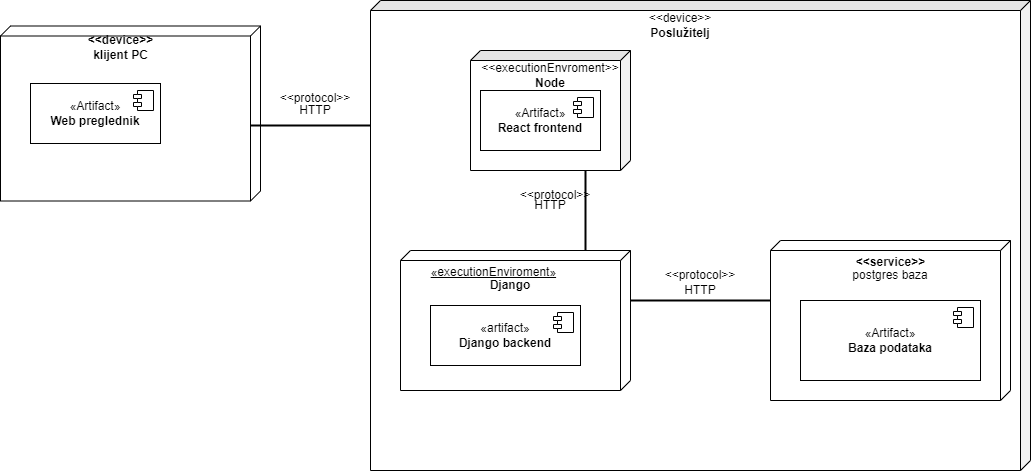
\includegraphics[scale=0.3]{dijagrami/Dijagram_razmjestaja.drawio.png}
				\caption{dijagram razmještaja}
				\label{fig:razmjestaj}
			\end{figure}
			
			
			\eject 
		
		\section{Upute za puštanje u pogon}
			
			%\textbf{\textit{dio 2. revizije}}\\
		
			 %\textit{U ovom poglavlju potrebno je dati upute za puštanje u pogon (engl. deployment) ostvarene aplikacije. Na primjer, za web aplikacije, opisati postupak kojim se od izvornog kôda dolazi do potpuno postavljene baze podataka i poslužitelja koji odgovara na upite korisnika. Za mobilnu aplikaciju, postupak kojim se aplikacija izgradi, te postavi na neku od trgovina. Za stolnu (engl. desktop) aplikaciju, postupak kojim se aplikacija instalira na računalo. Ukoliko mobilne i stolne aplikacije komuniciraju s poslužiteljem i/ili bazom podataka, opisati i postupak njihovog postavljanja. Pri izradi uputa preporučuje se \textbf{naglasiti korake instalacije uporabom natuknica} te koristiti što je više moguće \textbf{slike ekrana} (engl. screenshots) kako bi upute bile jasne i jednostavne za slijediti.}
			
			
			 %\textit{Dovršenu aplikaciju potrebno je pokrenuti na javno dostupnom poslužitelju. Studentima se preporuča korištenje neke od sljedećih besplatnih usluga: \href{https://aws.amazon.com/}{Amazon AWS}, \href{https://azure.microsoft.com/en-us/}{Microsoft Azure} ili \href{https://www.heroku.com/}{Heroku}. Mobilne aplikacije trebaju biti objavljene na F-Droid, Google Play ili Amazon App trgovini.}
			
			Upute podrazumijevaju da je slijedeće podešeno prije puštanja u pogon:
			\begin{itemize}
				\item Podešen PostgreSQL poslužitelj i pgadmin4 tako da mogu međusobno komunicirati
				\item Podešena instalacija Python-a 3.10 ili novijeg na razini sustava
				\item Podešena node.js instalacija s instaliranim upraviteljem paketa npm
				\item Podešen poslužitelj na način da je javno dostupan i komunikacija među portovima 3000 i 8000 nije onemogućena vatrozidom
			\end{itemize}	
			Napomena: Sljedeće upute će postaviti aplikaciju tako da se procesi Django, React i PostgreSQL izvršavaju na istom računalu
			
			Koraci:
			\begin{packed_enum}
				\item Otvorite naredbeni redak (cmd.exe ili terminal)
				\item Izvršite naredbu: git clone https://github.com/glatkobrasno/wall-e-zohari
				\item Komanda generira cijelo stablo direktorija, uključujući frontend (react) i backend (django) dijelove koda.
				Zatim se prebacite u backend direktorij koji je nastao prethodnom naredbom. Komanda: \\ cd  ./wall-e-zohari/IzvorniKod/backend/KuhajIT
				\item Napunite podatke u PostgreSQL bazu korištenjem pgadmin4 programom. Podatci za punjenje baze se nalaze u backend/KuhajIT direktoriju, KuhajITDatabase.sql. 
				\item Zatim se instalira i aktivira python virtualno okruženje, te instalitaju potrebni paketi komandama:
				\item[] \begin{packed_enum}
				    \item pip install virtualenv
				    \item virtualenv ../venv
     				\item ..\textbackslash venv\textbackslash Scripts\textbackslash activate.bat - u Windows okruženju
      				\item source ../venv/bin/activate - u Linux okruženju

				    \item pip install -r requirements.txt	
				\end{packed_enum}
				\item Podesiti varijable okruženja editiranjem datoteke \\ ./wall-e-zohari/IzvorniKod/backend/KuhajIT/KuhajIT/.env
				\item Sadržaj datoteke je opisan na glavnoj stranici repozitorija.
			     \item Pokrenuti django server komandom: 
				\item[] \begin{verbatim}
				nohup python manage.py runserver_plus 0.0.0.0:8000 --cert-file self.crt --key-file self.key 2> &1 >>django.log &     - u Linux okruženju
				python manage.py runserver_plus 0.0.0.0:8000 --cert-file self.crt --key-file self.key     - u Windows okruženju
				\end{verbatim}
			     \item pokrenuti react server komandama:
			     \item[] \begin{packed_enum}
			     	\item cd ./wall-e-zohari/IzvorniKod/frontend/my-app
			     	\item npm install yarn
			     	\item npm install
			     	\item npm run build
			     	
			     	\item \begin{verbatim}nohup node server.js  2> & 1 >react.log &         - u Linux okruženju
			     	\end{verbatim}
			     	\item node server.js   - u Windows okruženju
				\end{packed_enum}
				\item U ovom trenutku bi trebale biti pokrenute sve komponente sustava.
				\item django poslužuje na IP adresi localhost na portu 8000
				\item react poslužuje na IP adresi localhost na portu 3000
				\item PostgreSQL poslužuje na IP adresi localhost na portu 5432
				
				
			\eject 